\documentclass[14pt,a4paper]{scrartcl}
\usepackage[utf8]{inputenc}
\usepackage[english,russian]{babel}
\usepackage{indentfirst}
\usepackage{misccorr}
\usepackage{graphicx}
\usepackage{amsmath}
\usepackage{textcomp}
\usepackage{alltt}
\usepackage{amssymb}
\usepackage{pgfplots}
\graphicspath{{pictures/}}
\begin{document}
\begin{titlepage}
  \begin{center}
    \large
    МИНИСТЕРСТВО ОБРАЗОВАНИЯ И НАУКИ\\ РОССИЙСКОЙ ФЕДЕРАЦИИ
     
    \vspace{0.5cm}
 
    Федеральное государственное автономное образовательное учреждение высшего образования \\ «МОСКОВСКИЙ ФИЗИКО-ТЕХНИЧЕСКИЙ ИНСТИТУТ (научно-исследовательский институт)»
    \vspace{0.25cm}

	Физтех-школа аэрокосмических технологий
     
    Кафедра общей физики
    \vfill
     
     

    Голубятников Сергей
    \vfill
 
    \textsc{Отчёт по лабораторной работе}\\[5mm]
     
    {\LARGE Эффект Рамзауэра}
  \bigskip
     
   3 курс, группа Б03-903
\end{center}
\vfill
 
\newlength{\ML}
\settowidth{\ML}{«\underline{\hspace{0.7cm}}» \underline{\hspace{2cm}}}
\hfill
\begin{minipage}{0.4\textwidth}
  Руководитель работы\\
  \underline{\hspace{\ML}} Л.\,В.~Инжечик\\
  «\underline{\hspace{0.7cm}}» \underline{\hspace{2cm}} 2021 г.
\end{minipage}%
\bigskip
 

\vfill
 
\begin{center}
  Долгопрудный, 2021 г.
\end{center}
\end{titlepage}


\tableofcontents
\addcontentsline{exp}{section}{Заголовок добавить в содержание}
\newpage


\section{Цель работы}

Исследовать энергетическую зависимость вероятности рассеяния электронов атомами ксенона, определить энергии электронов, при которых наблюдается "просветление" ксенона, и оценить размер его внешней электронной оболочки.

\section{В работе используются:}
Тиратрон ТГ3-01/1.3Б, заполненный инертным газом, осциллограф, вольтметры.





\section{Теория}
К. Рамзауэр в 1921 г. исследовал зависимость поперечных сечений упругого рассеяния электронов (с энергией до 10 эВ) на атомах аргона. В результате этих исследований было обнаружено явление, получившее название эффекта Рамзауэра. \\

Эффективное сечение реакции (иногда его называют поперечным сечением или просто сечением реакции) — это величина, характеризующая вероятность перехода системы двух сталкивающихся частиц в результате их рассеяния (упругого или неупругого) в определенное конечное состояние. Сечение $\sigma$ равно отношению числа $N$ таких переходов в единицу времени к плотности $nv$ потока рассеиваемых частиц, падающих на мишень, т. е. к числу частиц, проходящих в единицу времени через единичную площадку, перпендикулярную к их скорости $v$ ($n$ — плотность числа падающих частиц)
\begin{equation}
\sigma = \frac{N}{nv}
\end{equation}
Таким образом, сечение имеет размерность площади. \\


\begin{figure}[h]
\begin{center}
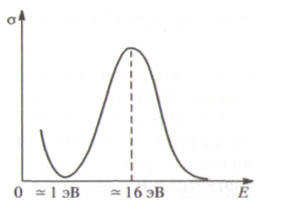
\includegraphics[width = 0.5\textwidth]{graph.png}
\caption{Качественная картина результатов измерения упругого рассеяния электронов в аргоне}
\end{center}
\end{figure}






Качественно результат экспериментов Рамзауэра при энергии электронов порядка десятков электрон-вольт на аргоне показан на рис. \ref{graph}. По мере уменьшения энергии электрона от нескольких десятков электрон-вольт поперечное сечение его упругого рассеяния растет, как это и следует из очень проcтых рассуждений: чем меньше скорость электрона, тем медленнее он "проскакивает" мимо атома, тем больше время взаимодействия электронов с атомом и, тем самым, больше вероятность этого взаимодействия, т. е. сечение реакции. Однако в эксперименте наблюдалось, что при энергиях меньше 16 эВ сечение начинает уменьшаться, а при $E \sim $ 1 эВ практически равно нулю, т. е. аргон становится прозрачным для электронов. При дальнейшем уменьшении энергии электронов сечение рассеяния опять начинает возрастать. Объяснение этого эффекта требует  учета волновой природы электронов. \\




\begin{figure}[h]
\begin{center}
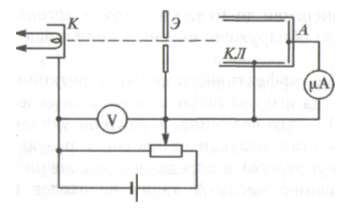
\includegraphics[width = 0.5\textwidth]{scheme.png}
\caption{Схема установки для измерения сечения рассеяния электронов в газах}
\end{center}
\end{figure}





Схема эксперимента Рамзауэра показана на рис. \ref{scheme}.
Пучок электронов, вылетая из накаленного катода К, проходит ускоряющую разность потенциалов V, приложенную между катодом и электродом Э, и приобретает тем самым энергию $E = m v^2 /2 = eV$. При прохождении через газ часть электронов рассеивается на атомах, уходит в сторону и собирается коллектором КЛ, а прошедшие без рассеяния электроны попадают на анод А и создают анодный ток $I$. Ток $I$ пропорционален числу прошедших электронов, и поэтому непосредственно характеризует проницаемость газа для электронного пучка в зависимости от его скорости (ускоряющего напряжения). Согласно классическим воззрениям, с ростом напряжения V, как указывалось выше, сечение рассеяния уменьшается, и ток должен монотонно возрастать. \\

С точки зрения квантовой теории картина рассеяния выглядит иначе. Внутри атома потенциальная энергия налетающего электрона $U$ отлична от нуля, скорость электрона изменяется, становясь равной $v'$ в соответствии с законом сохранения энергии
\begin{equation}
E = \frac{m v^2}{2} = \frac{m v'^2}{2} + U,
\end{equation}
а значит, изменяется и его длина волны де Бройля. Таким образом, по отношению к электронной волне атом ведет себя как преломляющая среда с относительным показателем преломления
\begin{equation}
n = \frac{\lambda}{\lambda'} = \sqrt{1 - \frac{U}{E}}.
\end{equation}




\begin{figure}[h]
\begin{center}
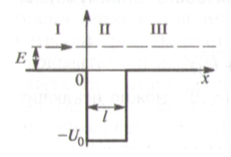
\includegraphics[width = 0.5\textwidth]{problem.png}
\caption{Схематическое изображение прямоугольной ямы, над которой пролетает частица с энергией $E$}
\end{center}
\end{figure}






Для качественного анализа вопроса рассмотрим следующую модель: будем считать, что электрон рассеивается на одномерной потенциальной яме конечной глубины. Форму ямы для качественных оценок можно считать прямоугольной. Модель прямоугольной потенциальной ямы является хорошим приближением для атомов тяжелых инертных газов, отличающихся наиболее компактной структурой и резкой внешней границей.

Уравнение Шредингера в данном случае имеет вид:
\begin{equation}
\psi'' + k^2 \psi = 0, 
\end{equation}
где
\begin{equation}
k^2 = 
\begin{cases}
k_1^2 = \frac{2mE}{\hbar^2} & \text{ - в областях I и III}\\
k_2^2 = \frac{2m(E+U_0)}{\hbar^2} & \text{ - в области II}
\end{cases}
\end{equation}

Коэффициент прохождения равен отношению квадратов амплитуд прошедшей и падающей волн и определяется выражением
\begin{equation}
D^{-1} = 1 + \frac{(k_1^2 - k_2^2)^2}{4k_1^2 k_2^2} \sin^2(k_2l) = 1 + \frac{U_0^2}{4E(E+U_0)} \sin^2(k_2l)
\end{equation}



\begin{figure}[h]
\begin{center}
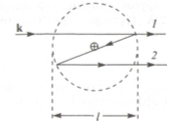
\includegraphics[width = 0.5\textwidth]{wave.png}
\caption{Схема интерференции волн де Бройля при рассеянии на атоме}
\end{center}
\end{figure}







Мы видим, что коэффициент прохождения частицы над ямой имеет, в зависимости от ее энергии, ряд чередующихся максимумов и мини мумов. В частности, если $k_2l = \pi$, то $\sin k_2l = 0$ и коэффициент прохож дения равен единице, т. е. отраженная волна отсутствует, и электрон беспрепятственно проходит через атом, что является квантовым аналогом просветления оптики.
Таким образом, коэффициент прохождения электронов максимален при условии 
\begin{equation}
k_2l = \sqrt{\frac{2m(E+U_0)}{\hbar^2}}l = \pi n, n = 1, 2, 3...
\end{equation}

Это условие можно легко получить, рассматривая интерференцию электронныъ волн де Бройля в атоме. Движущемуся электрону соответствует волна де Бройля, длина которой определяется соотношением $\lambda  = h/mv$. Если кинетическая энергия электрона невелика, то $E = mv^2/2$ и $\lambda = h/\sqrt{2mE}$. При движении электрона через атом длина волны де Бройля становится меньше и равна $\lambda' = h/\sqrt{2m(E + U_0)}$, где $U_0$ — глубина атомного потенциала. При этом, как показано на рис. \ref{wave}, волна де Бройля отражается от границ атомного потенциала, т. е. от поверхно стиатома, и происходит интерференция прошедшей через атом волны и волны 2, отраженной от передней и задней границы атома (эти волны когерентны).

Прошедшая волна 1 усилится волной 2, если геометрическая разность хода между ними $\Delta = 2l = \lambda'$, что соответствует условию первого интерференционного максимума, т. е. при условии
\begin{equation} \label{max}
2l = \frac{h}{\sqrt{2m(E_1 + U_0)}}
\end{equation}
Здесь $E_1$ -- энергия электрона, соответствующая этому условию.

С другой стороны, прошедшая волна ослабится, если $\Delta = 2l = (3/2)\lambda'$, т.е. при условии 
\begin{equation} \label{min}
2l = \frac{3}{2} \frac{h}{\sqrt{2m(E_2 + U_0)}}
\end{equation}

Решая совместно эти два уравнения, можно исключить $U_0$ и найти эффективный размер атома $l$
\begin{equation} \label{size}
l = \frac{h \sqrt{5}}{\sqrt{32m(E_2 - E_1)}}
\end{equation}

Понятно, что энергии $E_1$ и $E_2$ соответствует энергиям электронов, прошедших разность потенциалов $V_1$ и $V_2$, т.е. $E_1 = eV_1$ и $E_2 = eV_2$. 

Из формул (\ref{max}) и (\ref{min}) можно также по измеренным величинам $E_1$ и $E_2$ рассчитать эффективную глубину потенциальной ямы атома:
\begin{equation} \label{hole}
U_0 = \frac{4}{5} E_2 - \frac{9}{5} E_1
\end{equation}


\section{Экспериментальная установка}

\begin{figure}[ht!]\label{tiratron} 
 \center{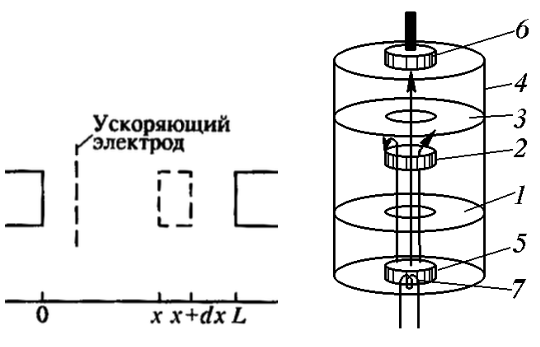
\includegraphics[width=.6\linewidth]{tiratron.png}}
\caption{Схематическое изображение тиратрона (слева) и его конструкция (справа): 1, 2, 3 - сетки; 4 -- внешний металлический цилиндр; 5 -- катод; 6 -- анод; 7 -- накаливаемая спираль}
\end{figure}

Уравнение ВАХ тиратрона:
\begin{equation} \label{VAH}
I_a = I_0 e^{-C\omega(V)}, C = L n_a \Delta_a,
\end{equation}
где $I_0 = e N_0$ -- ток катода, $I_a = e N_a$ -- анодный ток, $\omega(V)$ -- вероятность рассеяния электрона на атоме, $\Delta_a$ -- площадь попереченого сечения атома, $n_a$ -- концентрация атомов газа в лампе, $N_0$ -- поток электронов у катода, $N_a$ -- поток электронов у анода, $L$ -- длина лампы.


\begin{figure}[ht!]\label{omega} 
 \center{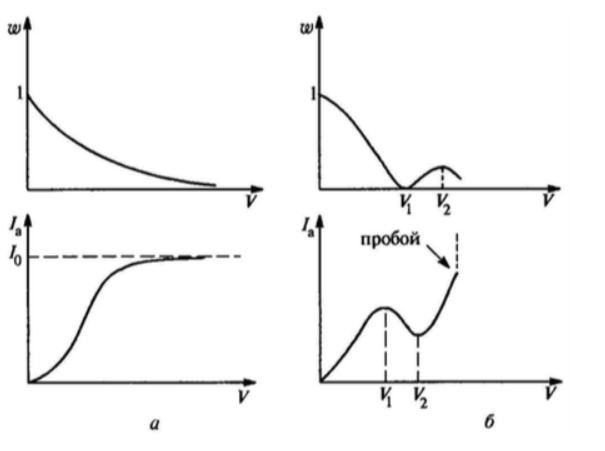
\includegraphics[height=30ex]{omega_teor.png}}
\caption{Качественный вид вероятности рассеяния электрона атомом инертного газа и ВАХ тиратрона при классическом (а) и квантовом (б) рассмотрении}
\end{figure}

Согласно классическим представлениям сечение рассеяния электрона на атоме должно падать монотонно с ростом V (обратно пропорционально скорости электрона, т. е. обратно пропорционально квадратному корню из его энергии), а значит, ВАХ будет монотонно возрастающей функцией, как это показано на рис. 6а. По квантовым соображениям вероятность рассеяния электронов и соответствующая ВАХ должны иметь вид, показанный на рис. 66.

Согласно формуле (\ref{VAH}) по измеренной ВАХ тиратрона можно определить зависимость вероятности рассеяния электрона от его энергии из соотношения
\begin{equation}
\omega(V) = -\frac{1}{C} \log\frac{I_a(V)}{I_0}
\end{equation}



\section{Ход работы}


Снимем ВАХ тиратрона в динамическом режиме для двух напряжений. Погрешности величин:  $\sigma_{V_{\text{катод-сетка}}} = 0.001$В, $\sigma_{V_{\text{анод-сетка}}} = 0.01$В, $\sigma_{I_{\text{анода}}} = 0.1$мкА.

\begin{figure}[ht!]
 \center{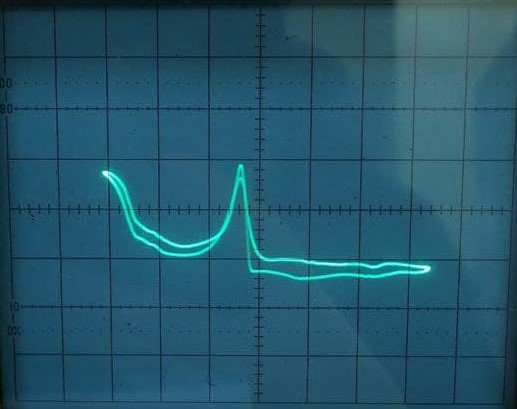
\includegraphics[height=35ex]{2_5.jpg}}
\caption{2.5 B}
\end{figure}


Определим $V_{min}$ и $V_{max}$:


$$V_{min} = 7.0 \pm 0.5 \text{ В}$$ 
$$V_{max} = 2.0 \pm 0.5 \text{ В}$$ 


Окгруглил погрешности, так как очень сильно плавали цифры на приборе.  
Оценим ионизационный потенциал газа. Полученное значение $V_{проб} \approx 11.5 \pm 0.5$ В хорошо совпаедет и укладывается в погрешность оценки напряжения пробоя ксенона $V_{ксенон} = 12.1$В. Значит, газ внутри - ксенон.

Снимем ВАХ в статическом режиме для двух напряжений накала: 2,5 В и 2 В (рис. 8, 9).

(Данные для графиков смотреть в приложении)

\begin{figure}[ht!]\label{omega} 
 \center{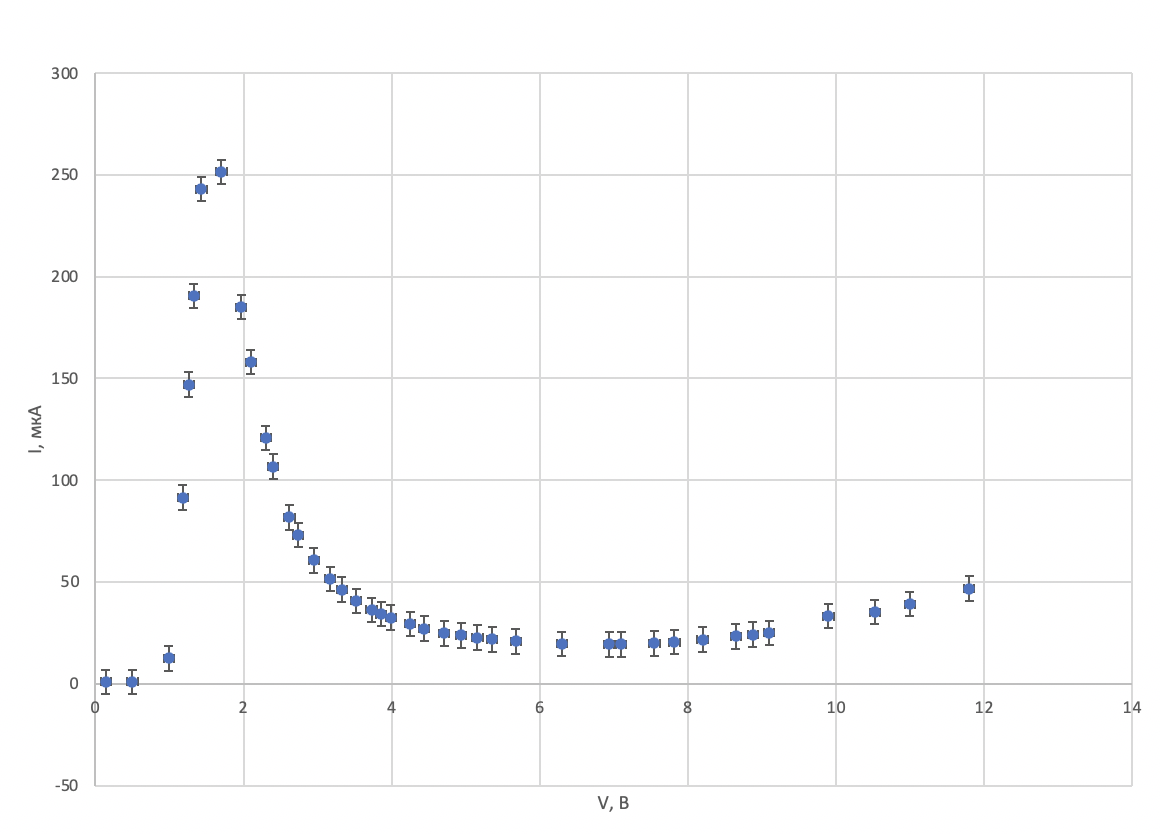
\includegraphics[scale = 0.45]{Screenshot 2021-11-21 at 20.09.57.png}}
\caption{ВАХ тиратрона, $V_{\text{накала}}=2$В}
\end{figure}



\begin{figure}[ht!]\label{omega} 
 \center{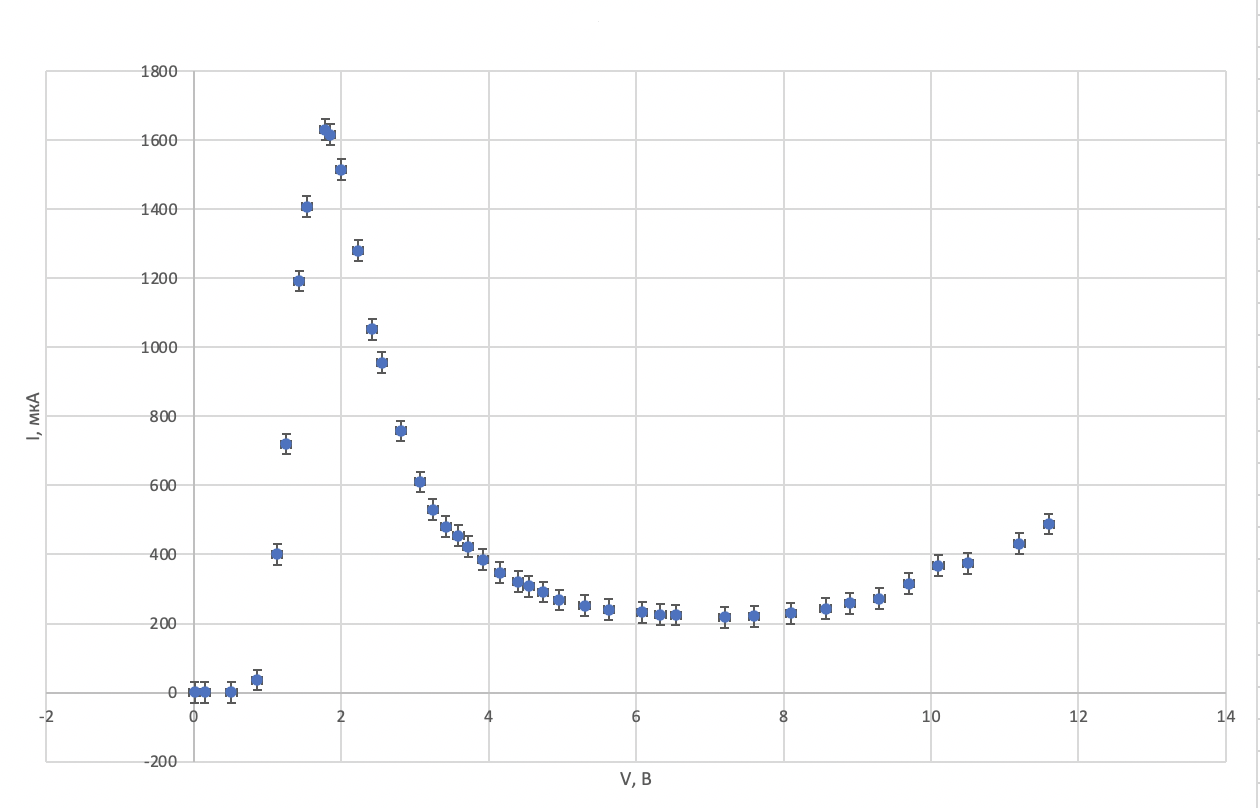
\includegraphics[scale = 0.45]{Screenshot 2021-11-21 at 20.08.48.png}}
\caption{ВАХ тиратрона, $V_{\text{накала}}=2,5$В}
\end{figure}




\newpage
\newpage

Полученное напряжение пробоя $V_\text{проб} \approx 11.7 \pm 0.5 B$  совпадает с напряжением пробоя ксенона в пределах погрешности $V_\text{ксенон} = 12.1 B$. Значит, что в тиратроне ксенон.\\


По графикам определим:

$$V_{min} \approx (6.5 \pm 0.2) B; \text{ } V_{max} \approx (1.8 \pm 0.2) B$$


По формуле (\ref{max}) для эффективного размера атома:

$$l = \frac{h}{2\sqrt{2m(E_1 + U_0)}} \approx (3,3 \pm 0.3) \text{{\AA}} $$ 

Погрешность:

$$\sigma_l = \left(\frac{h \sqrt{5}}{2\cdot \sqrt{32\cdot m}(V_{min} - V_{max})^{3/2}}\right) \sqrt{ (\sigma^2_{V_{min}} + \sigma^2_{V_{max}}})$$


По формуле (\ref{hole}) для глубины потенциальной ямы атома:
$$U_0 = \frac{4}{5} E_2 - \frac{9}{5} E_1 \approx (2.2 \pm 0.2) \text{эВ}$$
 
Погрешность:


$$
\sigma^2_{U_0} = \frac{16}{25}\cdot \sigma^2_{E_{min}} + \frac{81}{25}\cdot \sigma^2_{E_{max}}
$$



\item Оценим положения следующих максимумов:

$$k_2l = \sqrt{\frac{2m(E_n+U_0)}{\hbar^2}}l = \pi n, n = 1, 2, 3...$$ 

$$\sqrt{\frac{E_n + U_0}{E_1 + U_0}} = n \Rightarrow E_n = (E_1 + U_0) n^2 - U_0$$

$$E_2 = 13 \text{ эВ}, E_3 = 32 \text{ эВ}, E_4= 59 \text{ эВ}$$ 

При таких энергиях электронов происходит ионизация газа.\\

Построим график зависимости $\omega(V)$ (рис. 10):

\begin{figure}[ht!]\label{omega} 
 \center{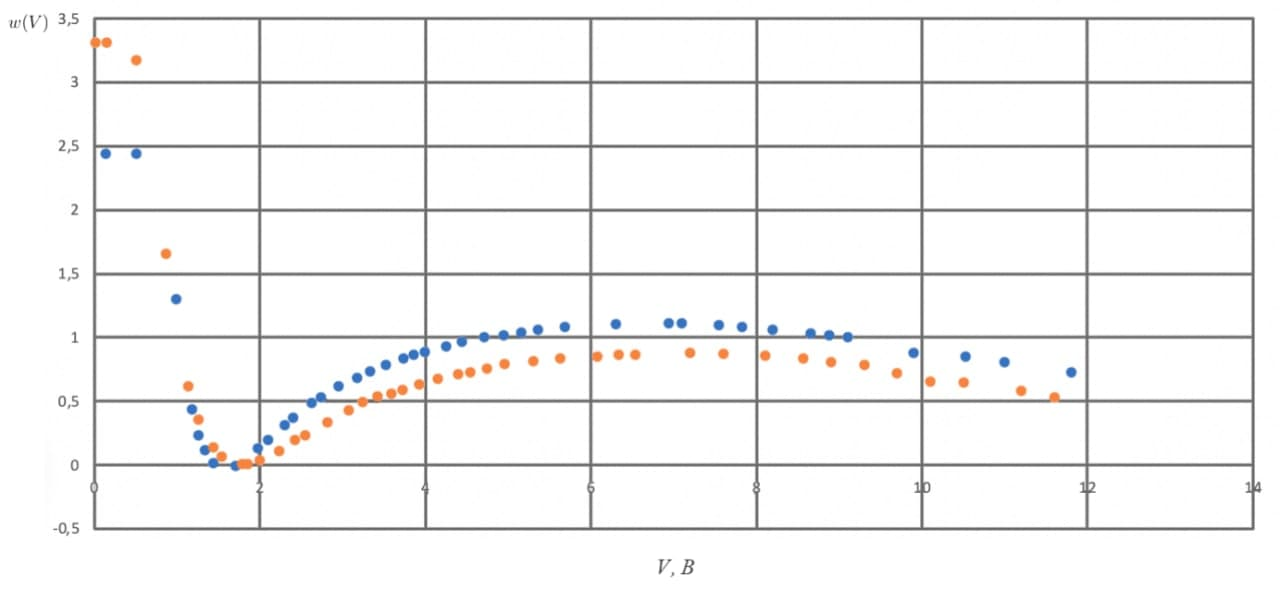
\includegraphics[width=.95\linewidth]{123.jpg}}
\caption{Зависимость вероятности рассеяния электрона на атоме от его энергии}
\end{figure}
 

\newpage

\section{Вывод}


В ходе лабораторной работы провел опыты по изучению рассеяния медленных электронов. Наблюдал ВАХ тиратрона в динамическом режиме при различных напряжениях накала. Определил напряжение пробоя $V_{\text{проб}} \approx 11.7 \pm 0.5 B$, что близко к табличному $V_{\text{табл}} = 12.1 B$. Из полученных данных получилось, что инертный газ - это ксенон. Был построен график зависимости вероятности рассеяния электрона на атоме от его энергии.



\addcontentsline{toc}{section}{Список используемой литературы}


\begin{thebibliography}{}

\bibitem{Sulsky1994}
Лабораторный практикум по общей физике: Учеб. пособие для вузов. Т. 3. Квантовая физика / Игошин Ф.Ф., Самарский Ю.А., Ципенюк Ю.М.; Под ред. Ципенюка Ю.М. - М.:Физматкнига, 2005. 432 стр.


\newpage

\section{Приложение}
В таблицах x - I, mA; y - V, B
	
\end{thebibliography}



		\begin{table}[h!]
		\caption{Таблица для V = 2B}
		\begin{center}
			\begin{tabular}{|c|c|p{15mm}|c|c|c|c|c|c|c|c|c|c|}
				\hline 
			x& 0,149 & 0,286 & 0,627 & 0,869 & 1,103 & 1,458 & 1,489 & 1,612 & 1,847 \\ 
			y & 1,733 & 2,344 & 3,906 & 6,250 & 63,500 & 104,688 & 186,719 & 221,875 & 256,250  \\ \hline
			x & 1,946 & 2,197 & 2,229 & 2,392 & 2,564 & 2,788 & 3,093 & 3,109 & 3,500  \\ 
			y & 251,563 & 237,500 & 198,438 & 179,688 & 150,000 & 121,875 & 95,313 & 90,625 & 75,563  \\ \hline
			x & 3,775 & 3,866 & 3,906 & 4,246 & 4,320 & 4,626 & 4,775 & 5,021 & 5,393  \\
			y & 71,875 & 65,625 & 60,938 & 56,250 & 54,688 & 50,000 & 46,875 & 43,750 & 40,625  \\\hline
			x & 5,780 & 6,266 & 6,438 & 6,516 & 7,142 & 7,736 & 8,123 & 8,614 & 8,925  \\
			y & 37,500 & 34,375 & 32,813 & 32,813 & 32,344 & 33,594 & 34,375 & 35,938 & 37,500  \\\hline
			x & 9,241 & 9,844 & 10,238 & 10,476 & 11,509 & 11,874 &  &  &   \\
			y & 43,750 & 48,438 & 59,375 & 60,938 & 65,625 & 75,000 &  &  &   \\
				\hline 
			\end{tabular} 
		\end{center}
		\label{table_mn}
	\end{table}





		\begin{table}[h!]
		\caption{Таблица для V = 2.5B}
		\begin{center}
			\begin{tabular}{|c|c|c|c|c|c|c|c|c|c|c|c|c|}
				\hline 
			 x & 0,122 & 0,238 & 0,584 & 0,853 & 1,101 & 1,376 & 1,451 & 1,555   \\
			 y & 11,090 & 16,911 & 26,716 & 40,642 & 400,070 & 673,292 & 1196,541 & 1422,262   \\ \hline
			 
			 x & 1,760 & 1,832 & 2,077 & 2,213 & 2,358 & 2,473 & 2,739 & 3,002   \\
			 y & 1643,490 & 1614,587 & 1524,832 & 1270,640 & 1151,388 & 963,651 & 781,950 & 613,621    \\ \hline
			 
			 x & 3,104 & 3,389 & 3,733 & 3,829 & 3,902 & 4,165 & 4,309 & 4,556   \\
			 y & 580,190 & 494,453 & 461,669 & 421,470 & 390,123 & 363,234 & 350,442 & 322,803     \\ \hline
			 
			 x & 4,724 & 4,954 & 5,286 & 5,735 & 6,174 & 6,361 & 6,452 & 7,119    \\
			 y & 301,211 & 282,683 & 264,286 & 241,767 & 223,696 & 213,066 & 212,584 & 207,923    \\ \hline
			 
			 x & 7,760 & 8,110 & 8,606 & 8,882 & 9,218 & 9,792 & 10,189 & 10,378    \\
			 y & 218,022 & 220,501 & 230,311 & 244,108 & 280,914 & 312,088 & 381,960 & 393,904    \\ \hline
			 
			 x & 11,449 &  &  &  &  &  &  &  &      \\
			 x & 480,379 &  &  &  &  &  &  &  &      \\

			 
				\hline 
			\end{tabular} 
		\end{center}
		\label{table_mn}
	\end{table}

\begin{center}
\begin{table}[]
\begin{tabular}{rrlrr}
I , mA & V, B  &  & I , mA & V, B  \\
0,122  & 3,618 &  & 0,055  & 2,267 \\
0,638  & 3,732 &  & 0,605  & 2,233 \\
0,834  & 3,543 &  & 0,825  & 2,133 \\
0,913  & 1,728 &  & 0,935  & 1,067 \\
1,101  & 0,614 &  & 1,155  & 0,400 \\
1,266  & 0,958 &  & 1,265  & 0,200 \\
1,431  & 0,508 &  & 1,485  & 0,133 \\
1,645  & 0,552 &  & 1,705  & 0,067 \\
1,870  & 0,718 &  & 1,925  & 0,026 \\
1,992  & 0,967 &  & 2,035  & 0,065 \\
2,197  & 1,066 &  & 2,255  & 0,130 \\
2,313  & 0,278 &  & 2,475  & 0,195 \\
2,428  & 0,458 &  & 2,585  & 0,234 \\
2,573  & 0,980 &  & 2,695  & 0,325 \\
2,639  & 0,740 &  & 2,805  & 0,455 \\
2,972  & 1,124 &  & 3,135  & 0,520 \\
3,104  & 0,458 &  & 3,355  & 0,546 \\
3,389  & 1,391 &  & 3,575  & 0,650 \\
3,633  & 0,884 &  & 3,905  & 0,715 \\
3,729  & 0,894 &  & 4,015  & 0,780 \\
3,902  & 0,675 &  & 4,235  & 0,845 \\
4,265  & 1,347 &  & 4,565  & 0,910 \\
4,609  & 0,868 &  & 5,005  & 1,014 \\
4,856  & 1,371 &  & 5,225  & 1,053 \\
4,924  & 1,082 &  & 5,335  & 1,092 \\
5,004  & 1,397 &  & 5,39   & 1,118 \\
5,386  & 1,747 &  & 5,775  & 1,157 \\
5,635  & 1,233 &  & 6,105  & 1,144 \\
6,274  & 1,649 &  & 6,765  & 1,183 \\
6,361  & 1,533 &  & 6,875  & 1,196 \\
6,452  & 1,447 &  & 6,985  & 1,209 \\
7,219  & 1,126 &  & 7,865  & 1,222 \\
7,810  & 1,524 &  & 8,47   & 1,196 \\
8,110  & 0,990 &  & 8,855  & 1,157 \\
8,406  & 0,922 &  & 9,185  & 1,118 \\
8,982  & 1,672 &  & 9,735  & 1,105 \\
9,118  & 1,043 &  & 9,955  & 1,118 \\
9,792  & 1,068 &  & 10,67  & 0,845 \\
10,239 & 1,022 &  & 11,165 & 0,819 \\
10,478 & 1,381 &  & 11,385 & 0,780 \\
11,249 & 1,065 &  & 12,265 & 0,754 \\
11,508 & 0,596 &  & 12,595 & 0,676
\end{tabular}
\end{table}

\end{center}

\end{document}